\documentclass[11pt, fleqn]{article}

\usepackage{amsmath}
\usepackage{amsfonts}
\usepackage{amsthm}
\usepackage[margin=1in]{geometry} % To set the margin widths
\usepackage{graphicx}
%\usepackage{hyperref}
\usepackage{listings}
\usepackage{multirow}
\usepackage{tabularx}
\usepackage{varioref}
\usepackage{cleveref}  % this redefines vref to use cleverref
\usepackage{siunitx}
%\usepackage{subcaption}
\usepackage{subfig}
\usepackage{titlesec}
\usepackage{bm}

\crefname{equation}{equation}{equations}
\crefname{figure}{figure}{figures}

\sisetup{output-exponent-marker=\textsc{e}}

\titleformat{\section}[block]{\bfseries}{\thesection}{1em}{}


\setlength{\parskip}{12pt} % Sets a blank line in between paragraphs
\setlength\parindent{0pt} % Sets the indent for each paragraph to zero

\begin{document}

\title{Big Data: Homework 6}
\author{Will Clark \& Matthew DeLio \\ 41201-01}
\date{\today}
\maketitle

\section{Node Connectivity Transformation}

\section{Appendix}
% latex table generated in R 3.1.2 by xtable 1.7-4 package
% Fri May 22 02:15:27 2015
\begin{table}[ht]
\centering
\begin{tabular}{rr}
  \hline
 & $\theta$ \\ 
  \hline
postal.service & 0.080 \\ 
  strong.support & 0.030 \\ 
  post.office & 0.029 \\ 
  endangered.speci.act & 0.029 \\ 
  passenger.rail & 0.028 \\ 
  drinking.water & 0.026 \\ 
  estate.tax & 0.024 \\ 
  appropriation.bil & 0.018 \\ 
  enemy.combatant & 0.018 \\ 
  water.act & 0.016 \\ 
   \hline
\end{tabular}
\caption{Non-Partisan Topic Words} 
\label{tab:non_part_topics}
\end{table}

% latex table generated in R 3.2.0 by xtable 1.7-4 package
% Fri May 22 07:11:37 2015
\begin{table}[ht]
\centering
\begin{tabular}{rrrr}
  \hline
 & $\log(\lambda)$ & $R^2$ & Covariates Selected \\ 
  \hline
AICc & -7.50 & 0.38 &  14 \\ 
  AIC & -7.50 & 0.38 &  14 \\ 
  BIC & -5.73 & 0.37 &  12 \\ 
  CV.Min & -7.50 & 0.34 &  14 \\ 
  CV.1se & -4.75 & 0.31 &  11 \\ 
   \hline
\end{tabular}
\caption{ICs for Republican Share $\sim$ Topic $\omega$} 
\label{tab:topic_repshare}
\end{table}

% latex table generated in R 3.1.2 by xtable 1.7-4 package
% Fri May 22 03:00:40 2015
\begin{table}[ht]
\centering
\begin{tabular}{rrrr}
  \hline
 & $\log(\lambda)$ & $R^2$ & Covariates Selected \\ 
  \hline
AICc & -2.78 & 0.24 &  32 \\ 
  AIC & -6.04 & 0.96 & 241 \\ 
  BIC & -2.27 & 0.08 &   6 \\ 
  CV.Min & -4.08 & 0.37 & 188 \\ 
  CV.1se & -3.20 & 0.29 &  92 \\ 
   \hline
\end{tabular}
\caption{ICs for Republican $\sim$ Phrase \%} 
\label{tab:repx}
\end{table}

% latex table generated in R 3.2.0 by xtable 1.7-4 package
% Fri May 22 07:11:36 2015
\begin{table}[ht]
\centering
\begin{tabular}{rrrrrr}
  \hline
 & \# Dem & \# Ind & \# Rep & Total & mean(RepShare) \\ 
  \hline
1 &  40 &   1 &   0 &  41 & 0.42 \\ 
  2 & 185 &   1 & 238 & 424 & 0.51 \\ 
  3 &   1 &   0 &   0 &   1 & 0.44 \\ 
  4 &   1 &   0 &   0 &   1 & 0.40 \\ 
  5 &   2 &   0 &   0 &   2 & 0.27 \\ 
  6 &   0 &   0 &   1 &   1 & 0.57 \\ 
  7 &   0 &   0 &   6 &   6 & 0.61 \\ 
  8 &   0 &   0 &  37 &  37 & 0.59 \\ 
  9 &   8 &   0 &   0 &   8 & 0.43 \\ 
  10 &   1 &   0 &   0 &   1 & 0.37 \\ 
  11 &   0 &   0 &   2 &   2 & 0.50 \\ 
  12 &   2 &   0 &   0 &   2 & 0.61 \\ 
  13 &   1 &   0 &   0 &   1 & 0.45 \\ 
  14 &   0 &   0 &   1 &   1 & 0.65 \\ 
  15 &   1 &   0 &   0 &   1 & 0.64 \\ 
   \hline
\end{tabular}
\caption{Cluster Summary for k=15 (min BIC)} 
\label{tab:k_means_summary}
\end{table}


\begin{figure}[!htb]
  \centering
  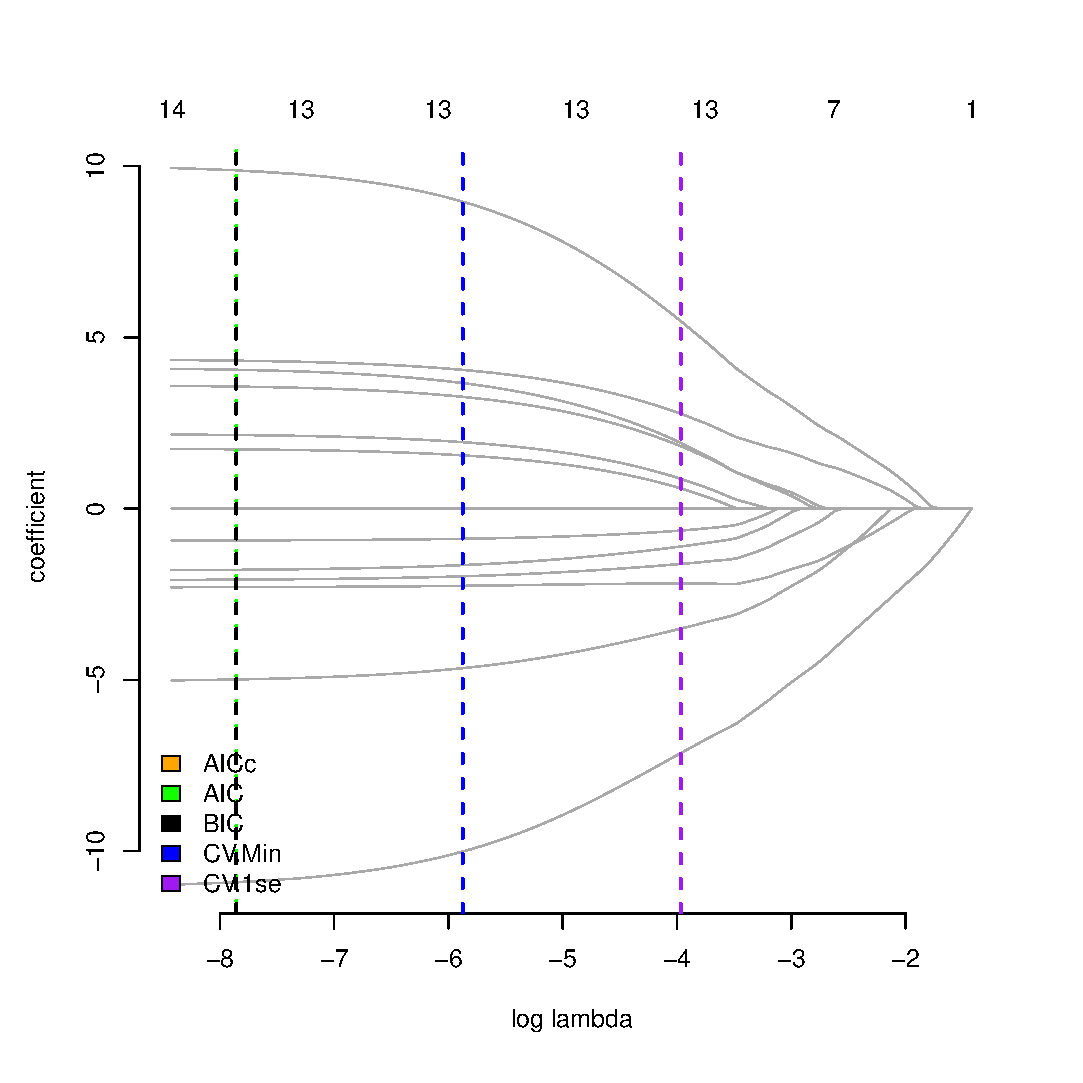
\includegraphics[scale=.5]{tpcs_rep.eps}
  \caption{Rep ~ $\Omega$ (Gamma Lasso Path with ICs)}
  \label{fig:}
\end{figure}

% latex table generated in R 3.2.0 by xtable 1.7-4 package
% Fri May 22 07:11:36 2015
\begin{table}[ht]
\centering
\begin{tabular}{rrrr}
  \hline
 & $\log(\lambda)$ & $R^2$ & Covariates Selected \\ 
  \hline
AICc & -7.86 & 0.56 &  13 \\ 
  AIC & -7.86 & 0.56 &  13 \\ 
  BIC & -7.86 & 0.56 &  13 \\ 
  CV.Min & -5.88 & 0.53 &  13 \\ 
  CV.1se & -3.97 & 0.50 &  13 \\ 
   \hline
\end{tabular}
\caption{ICs for Republican $\sim$ Topic $\omega$} 
\label{tab:topic_rep}
\end{table}


% \begin{figure}
%   \centering
%   \begin{subfigure}[b]{0.49\textwidth}
%     \includegraphics[width=\textwidth]{.eps}
%     \caption{}
%     \label{fig:}
%   \end{subfigure}
%   \hfill
%   \begin{subfigure}[b]{0.49\textwidth}
%     \includegraphics[width=\textwidth]{.eps}
%     \caption{}
%     \label{fig:}
%   \end{subfigure}
%   \caption{}
% \end{figure}


% \input{.tex}

% \begin{figure}
%   \centering
%   \begin{subfigure}[b]{0.49\textwidth}
%     \includegraphics[width=\textwidth]{.eps}
%     \caption{}
%     \label{fig:}
%   \end{subfigure}
%   \hfill
%   \begin{subfigure}[b]{0.49\textwidth}
%     \includegraphics[width=\textwidth]{.eps}
%     \caption{}
%     \label{fig:}
%   \end{subfigure}
%   \caption{}
% \end{figure}

% \begin{figure}[!htb]
%   \centering
%   \includegraphics[scale=.5]{.eps}
%   \caption{}
%   \label{fig:}
% \end{figure}

\end{document}